\documentclass[12pt,a4paper]{article}
\usepackage[utf8]{inputenc}
\usepackage[catalan]{babel}
\usepackage{graphicx}
\usepackage{geometry}
\usepackage{fancyhdr}
\usepackage{tabularx}
\usepackage{lastpage}
\usepackage{enumitem}
\usepackage{amsmath}
\usepackage{tikz}
\usepackage{tcolorbox}

\geometry{top=4cm, bottom=3cm, left=2cm, right=2cm, headheight=2.5cm}

\pagestyle{fancy}
\fancyhf{}
\fancyhead[L]{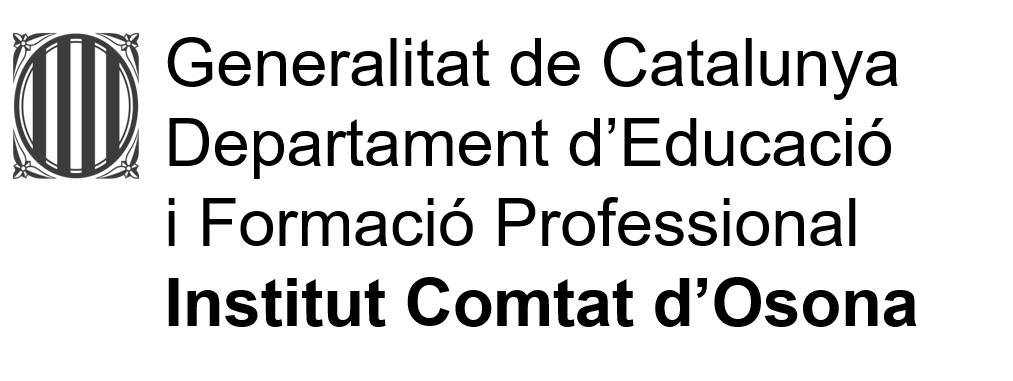
\includegraphics[height=1.8cm]{Logo_Departament.png}}
\fancyhead[R]{
\includegraphics[height=1.8cm]{Logo_Institut.png}}
\fancyfoot[C]{Pagina \thepage\ de \pageref{LastPage}}
\renewcommand{\headrulewidth}{0.4pt}

% ── Caixa buida per dibuixar ──────────────────────────────────────────────────
\newcommand{\dibuixabox}{%
  \begin{tikzpicture}[scale=0.72]
    \draw[dashed, gray!70] (0,0) rectangle (6.5,5);
    \node[gray!80, font=\small\itshape] at (3.25,2.5) {Dibuixa la figura aqui};
  \end{tikzpicture}%
}

\begin{document}

% ── Capcalera d'identificacio ──────────────────────────────────────────────────
\begingroup
\renewcommand{\arraystretch}{2.2}
\begin{tabularx}{\textwidth}{|X|p{4cm}|}
    \hline
    \textbf{Nom i cognoms:} & \textbf{Grup:} \\ \hline
    \textbf{Activitat:} Fitxa d'entrenament: Perimetres i Arees & \textbf{Data:} \\ \hline
\end{tabularx}
\endgroup

\vspace{0.4cm}

\begin{tcolorbox}[colback=yellow!5, colframe=yellow!70!black, title=Recordatori rapid]
\small
\textbf{Quadrat/Rectangle:} $P = \text{suma costats}$,\; $A = b \cdot h$
\quad|\quad
\textbf{Triangle:} $A = \dfrac{b \cdot h}{2}$ \\[4pt]
\textbf{Cercle:} $L = 2 \cdot \pi \cdot r$,\; $A = \pi \cdot r^2$
\quad (fes servir $\pi = 3{,}14$)
\end{tcolorbox}

\vspace{0.4cm}

% ================================================================================
%  EXERCICI 1 - QUADRILATERS
% ================================================================================
\section*{1. Quadril\`aters \normalfont\small(Dibuixa la figura i calcula el Per\'imetre i l'\'Area)}

% --- Fila 1 ---
\noindent
\begin{minipage}[t]{0.31\textwidth}
\centering
\textbf{a)} Quadrat $c = 4$ cm {\footnotesize\textit{(exemple)}}\\[4pt]
\begin{tikzpicture}[scale=0.72]
  \draw[thick] (0,0) rectangle (4,4);
  \node[below] at (2,0) {\small 4 cm};
  \node[left]  at (0,2) {\small 4 cm};
\end{tikzpicture}\\[6pt]
$P = 4 \times 4 = \mathbf{16}$ cm\\[4pt]
$A = 4 \times 4 = \mathbf{16}$ cm$^2$
\end{minipage}
\hfill
\begin{minipage}[t]{0.31\textwidth}
\centering
\textbf{b)} Rectangle $6 \times 3$ cm\\[4pt]
\dibuixabox\\[6pt]
$P = \underline{\hspace{3cm}}$\\[4pt]
$A = \underline{\hspace{3cm}}$
\end{minipage}
\hfill
\begin{minipage}[t]{0.31\textwidth}
\centering
\textbf{c)} Quadrat $c = 10$ m\\[4pt]
\dibuixabox\\[6pt]
$P = \underline{\hspace{3cm}}$\\[4pt]
$A = \underline{\hspace{3cm}}$
\end{minipage}

\vspace{0.5cm}\noindent\rule{\textwidth}{0.3pt}\vspace{0.4cm}

% --- Fila 2 ---
\noindent
\begin{minipage}[t]{0.31\textwidth}
\centering
\textbf{d)} Rectangle $7 \times 2$ cm\\[4pt]
\dibuixabox\\[6pt]
$P = \underline{\hspace{3cm}}$\\[4pt]
$A = \underline{\hspace{3cm}}$
\end{minipage}
\hfill
\begin{minipage}[t]{0.31\textwidth}
\centering
\textbf{e)} Rectangle $8 \times 4$ m\\[4pt]
\dibuixabox\\[6pt]
$P = \underline{\hspace{3cm}}$\\[4pt]
$A = \underline{\hspace{3cm}}$
\end{minipage}
\hfill
\begin{minipage}[t]{0.31\textwidth}
\centering
\textbf{f)} Quadrat $c = 5$ cm\\[4pt]
\dibuixabox\\[6pt]
$P = \underline{\hspace{3cm}}$\\[4pt]
$A = \underline{\hspace{3cm}}$
\end{minipage}

\newpage

% ================================================================================
%  EXERCICI 2 - TRIANGLES
% ================================================================================
\section*{2. Triangles \normalfont\small(Dibuixa la figura i calcula l'\'Area)}

% --- Fila 1 ---
\noindent
\begin{minipage}[t]{0.31\textwidth}
\centering
\textbf{a)} $b = 4$ cm,\; $h = 3$ cm {\footnotesize\textit{(exemple)}}\\[4pt]
\begin{tikzpicture}[scale=0.72]
  \draw[thick] (0,0) -- (4,0) -- (2,3) -- cycle;
  \draw[dashed] (2,0) -- (2,3);
  \draw (2,0) -- ++(0.2,0) -- ++(0,0.2) -- ++(-0.2,0);
  \node[below] at (2,0)   {\small $b = 4$ cm};
  \node[right] at (2.1,1.5) {\small $h = 3$ cm};
\end{tikzpicture}\\[6pt]
$A = \dfrac{4 \times 3}{2} = \mathbf{6}$ cm$^2$
\end{minipage}
\hfill
\begin{minipage}[t]{0.31\textwidth}
\centering
\textbf{b)} $b = 10$ m,\; $h = 6$ m\\[4pt]
\dibuixabox\\[6pt]
$A = \underline{\hspace{3cm}}$
\end{minipage}
\hfill
\begin{minipage}[t]{0.31\textwidth}
\centering
\textbf{c)} $b = 5$ cm,\; $h = 4$ cm\\[4pt]
\dibuixabox\\[6pt]
$A = \underline{\hspace{3cm}}$
\end{minipage}

\vspace{0.5cm}\noindent\rule{\textwidth}{0.3pt}\vspace{0.4cm}

% --- Fila 2 ---
\noindent
\begin{minipage}[t]{0.31\textwidth}
\centering
\textbf{d)} $b = 8$ m,\; $h = 5$ m\\[4pt]
\dibuixabox\\[6pt]
$A = \underline{\hspace{3cm}}$
\end{minipage}
\hfill
\begin{minipage}[t]{0.31\textwidth}
\centering
\textbf{e)} $b = 12$ cm,\; $h = 10$ cm\\[4pt]
\dibuixabox\\[6pt]
$A = \underline{\hspace{3cm}}$
\end{minipage}
\hfill
\begin{minipage}[t]{0.31\textwidth}
\centering
\textbf{f)} $b = 6$ m,\; $h = 7$ m\\[4pt]
\dibuixabox\\[6pt]
$A = \underline{\hspace{3cm}}$
\end{minipage}

\vspace{0.8cm}

% ================================================================================
%  EXERCICI 3 - CERCLES
% ================================================================================
\section*{3. Cercles \normalfont\small(Dibuixa la figura i calcula la Longitud i l'\'Area)}

% --- Fila 1 ---
\noindent
\begin{minipage}[t]{0.31\textwidth}
\centering
\textbf{a)} Radi $r = 2$ cm {\footnotesize\textit{(exemple)}}\\[4pt]
\begin{tikzpicture}[scale=0.72]
  \draw[thick] (2.5,2.5) circle (2);
  \draw[->, thick] (2.5,2.5) -- (4.5,2.5);
  \node[above] at (3.5,2.5) {\small $r = 2$ cm};
  \fill (2.5,2.5) circle (2.5pt);
\end{tikzpicture}\\[6pt]
$L = 2 \cdot 3{,}14 \cdot 2 = \mathbf{12{,}56}$ cm\\[4pt]
$A = 3{,}14 \cdot 2^2 = \mathbf{12{,}56}$ cm$^2$
\end{minipage}
\hfill
\begin{minipage}[t]{0.31\textwidth}
\centering
\textbf{b)} Radi $r = 5$ m\\[4pt]
\dibuixabox\\[6pt]
$L = \underline{\hspace{3cm}}$\\[4pt]
$A = \underline{\hspace{3cm}}$
\end{minipage}
\hfill
\begin{minipage}[t]{0.31\textwidth}
\centering
\textbf{c)} Radi $r = 1$ cm\\[4pt]
\dibuixabox\\[6pt]
$L = \underline{\hspace{3cm}}$\\[4pt]
$A = \underline{\hspace{3cm}}$
\end{minipage}

\vspace{0.5cm}\noindent\rule{\textwidth}{0.3pt}\vspace{0.4cm}

% --- Fila 2 ---
\noindent
\begin{minipage}[t]{0.31\textwidth}
\centering
\textbf{d)} Radi $r = 10$ m\\[4pt]
\dibuixabox\\[6pt]
$L = \underline{\hspace{3cm}}$\\[4pt]
$A = \underline{\hspace{3cm}}$
\end{minipage}
\hfill
\begin{minipage}[t]{0.31\textwidth}
\centering
\textbf{e)} Radi $r = 4$ cm\\[4pt]
\dibuixabox\\[6pt]
$L = \underline{\hspace{3cm}}$\\[4pt]
$A = \underline{\hspace{3cm}}$
\end{minipage}
\hfill
\begin{minipage}[t]{0.31\textwidth}
\centering
\textbf{f)} Radi $r = 3$ m\\[4pt]
\dibuixabox\\[6pt]
$L = \underline{\hspace{3cm}}$\\[4pt]
$A = \underline{\hspace{3cm}}$
\end{minipage}

\newpage

% ================================================================================
%  EXERCICI 4 - FIGURES COMPOSTES  (tots els dibuixos fets)
% ================================================================================
\section*{4. Figures Compostes \normalfont\small(Calcula el Per\'imetre i l'\'Area)}
\textit{Calcula l'area total sumant les parts i el perimetre sumant nomes el contorn exterior.}

\subsection*{A) Dos rectangles junts}

\noindent
\begin{minipage}[t]{0.31\textwidth}
\centering
\textbf{a)}\\[4pt]
\begin{tikzpicture}[scale=0.55]
  \draw[thick] (0,0) rectangle (3,2);
  \draw[thick] (3,0) rectangle (5,4);
  \node[below] at (1.5,0) {\small 3};
  \node[below] at (4,0)   {\small 2};
  \node[left]  at (0,1)   {\small 2};
  \node[right] at (5,2)   {\small 4};
\end{tikzpicture}\\[6pt]
$P = \underline{\hspace{2.8cm}}$\\[4pt]
$A = \underline{\hspace{2.8cm}}$
\end{minipage}
\hfill
\begin{minipage}[t]{0.31\textwidth}
\centering
\textbf{b)}\\[4pt]
\begin{tikzpicture}[scale=0.55]
  \draw[thick] (0,0) rectangle (5,2);
  \draw[thick] (1,2) rectangle (4,4);
  \node[below] at (2.5,0) {\small 5};
  \node[left]  at (0,1)   {\small 2};
  \node[above] at (2.5,4) {\small 3};
  \node[right] at (4,3)   {\small 2};
  \node[below] at (0.5,2) {\small 1};
  \node[below] at (4.5,2) {\small 1};
\end{tikzpicture}\\[6pt]
$P = \underline{\hspace{2.8cm}}$\\[4pt]
$A = \underline{\hspace{2.8cm}}$
\end{minipage}
\hfill
\begin{minipage}[t]{0.31\textwidth}
\centering
\textbf{c)}\\[4pt]
\begin{tikzpicture}[scale=0.55]
  \draw[thick] (0,0) -- (4,0) -- (4,4) -- (2,4) -- (2,2) -- (0,2) -- cycle;
  \node[below] at (2,0)   {\small 4};
  \node[right] at (4,2)   {\small 4};
  \node[above] at (3,4)   {\small 2};
  \node[left]  at (0,1)   {\small 2};
  \node[above] at (1,2)   {\small 2};
  \node[right] at (2,3)   {\small 2};
\end{tikzpicture}\\[6pt]
$P = \underline{\hspace{2.8cm}}$\\[4pt]
$A = \underline{\hspace{2.8cm}}$
\end{minipage}

\vspace{0.8cm}

\subsection*{B) Rectangle + Triangle}

\noindent
\begin{minipage}[t]{0.31\textwidth}
\centering
\textbf{a)}\\[4pt]
\begin{tikzpicture}[scale=0.55]
  \draw[thick] (0,0) rectangle (4,3);
  \draw[thick] (0,3) -- (2,5) -- (4,3);
  \draw[dashed] (2,3) -- (2,5);
  \node[below]  at (2,0)   {\small 4};
  \node[left]   at (0,1.5) {\small 3};
  \node[right]  at (2.1,4) {\small $h{=}2$};
\end{tikzpicture}\\[6pt]
$P = \underline{\hspace{2.8cm}}$\\[4pt]
$A = \underline{\hspace{2.8cm}}$
\end{minipage}
\hfill
\begin{minipage}[t]{0.31\textwidth}
\centering
\textbf{b)}\\[4pt]
\begin{tikzpicture}[scale=0.55]
  \draw[thick] (0,0) rectangle (3,4);
  \draw[thick] (3,0) -- (5,0) -- (3,4);
  \node[below] at (1.5,0)  {\small 3};
  \node[left]  at (0,2)    {\small 4};
  \node[below] at (4,0)    {\small 2};
\end{tikzpicture}\\[6pt]
$P = \underline{\hspace{2.8cm}}$\\[4pt]
$A = \underline{\hspace{2.8cm}}$
\end{minipage}
\hfill
\begin{minipage}[t]{0.31\textwidth}
\centering
\textbf{c)}\\[4pt]
\begin{tikzpicture}[scale=0.55]
  \draw[thick] (0,0) rectangle (6,2);
  \draw[thick] (2,2) -- (3,4) -- (4,2);
  \draw[dashed] (3,2) -- (3,4);
  \node[below] at (3,0)    {\small 6};
  \node[left]  at (0,1)    {\small 2};
  \node[right] at (3.1,3)  {\small $h{=}2$};
  \node[above] at (3,2)    {\small 2};
\end{tikzpicture}\\[6pt]
$P = \underline{\hspace{2.8cm}}$\\[4pt]
$A = \underline{\hspace{2.8cm}}$
\end{minipage}

\vspace{0.8cm}

\subsection*{C) Rectangle + Mitja circumfer\`encia}

\noindent
\begin{minipage}[t]{0.31\textwidth}
\centering
\textbf{a)}\\[4pt]
\begin{tikzpicture}[scale=0.55]
  % Rectangle (sense tapa superior)
  \draw[thick] (0,0) -- (4,0) -- (4,3) -- (0,3) -- cycle;
  % Semicercle a sobre (radi = 2, centrat a (2,3))
  \draw[thick] (4,3) arc (0:180:2);
  % Radi puntejat
  \draw[dashed] (2,3) -- (2,5);
  \fill (2,3) circle (2pt);
  \node[below] at (2,0)   {\small 4};
  \node[left]  at (0,1.5) {\small 3};
  \node[right] at (2.2,4) {\small $r{=}2$};
\end{tikzpicture}\\[6pt]
$P = \underline{\hspace{2.8cm}}$\\[4pt]
$A = \underline{\hspace{2.8cm}}$
\end{minipage}
\hfill
\begin{minipage}[t]{0.31\textwidth}
\centering
\textbf{b)}\\[4pt]
\begin{tikzpicture}[scale=0.55]
  % Rectangle
  \draw[thick] (0,0) rectangle (5,2);
  % Semicercle a la dreta (radi = 1, centrat a (5,1))
  \draw[thick] (5,0) arc (-90:90:1);
  % Radi puntejat
  \draw[dashed] (5,1) -- (6,1);
  \fill (5,1) circle (2pt);
  \node[below] at (2.5,0) {\small 5};
  \node[left]  at (0,1)   {\small 2};
  \node[right] at (6.1,1.3) {\small $r{=}1$};
\end{tikzpicture}\\[6pt]
$P = \underline{\hspace{2.8cm}}$\\[4pt]
$A = \underline{\hspace{2.8cm}}$
\end{minipage}
\hfill
\begin{minipage}[t]{0.31\textwidth}
\centering
\textbf{c)}\\[4pt]
\begin{tikzpicture}[scale=0.55]
  % Quadrat
  \draw[thick] (0,0) rectangle (2,2);
  % Semicercle a sobre (radi = 1, centrat a (1,2))
  \draw[thick] (2,2) arc (0:180:1);
  % Radi puntejat
  \draw[dashed] (1,2) -- (1,3);
  \fill (1,2) circle (2pt);
  \node[below] at (1,0)   {\small 2};
  \node[left]  at (0,1)   {\small 2};
  \node[right] at (1.2,2.5) {\small $r{=}1$};
\end{tikzpicture}\\[6pt]
$P = \underline{\hspace{2.8cm}}$\\[4pt]
$A = \underline{\hspace{2.8cm}}$
\end{minipage}

\end{document}